\section{ZK-ZKVM} \label{sec:zk-zkvm}

OlaVM \ref{section: olavm} is a ZK-VM which is a system that uses zk technology to implement a verifiable circuit system for general computation. However, it has some issues where privacy is required, for example, quotation data of commercial competition, anonymous auction, etc. The ZK-VM's each proof generation leaks the witness data, such as the name and function of the called contract, parameters, and so on.

To address this privacy concern, the ZK-ZKVM system has been developed. This system builds on top of ZK-VM but adds an extra layer of privacy by ensuring that all witness data is private and does not reveal any information. This is achieved through the use of different permissioned private key systems and a note mechanism similar to ZCash's UTXO model.

The core technology of ZK-ZKVM is the use of different permissioned private key systems. These keys are used to encrypt and decrypt the witness data, ensuring that it remains private and secure. Additionally, the note mechanism is used to further enhance the privacy of the system. Each note represents a commitment to a certain amount of value, and it is impossible to deduce any information about the transaction from this commitment.

The importance of ZK-ZKVM lies in its ability to address the privacy concerns that exist in ZK-VM. With ZK-ZKVM, users can conduct transactions on public blockchains with the assurance that their sensitive information is secure and private. This makes it suitable for a wide range of use cases that require high levels of privacy, such as financial transactions or data sharing.

Furthermore, ZK-ZKVM also offers the same scalability benefits as ZK-VM. By allowing for off-chain computation and verification, it reduces the burden on the main blockchain and increases transaction throughput. This makes it a more efficient and effective solution for blockchain scaling than traditional solutions.

In Section \ref{section: zkzkvm-framework} we explain our basic framework of ZK-ZKVM. Then, in Section \ref{section: zkzkvm-key}, we explain the key system design in our ZK-ZKVM system. Then, in Section \ref{section: zkzkvm-note}, we explain the note design in our ZK-ZKVM system. Then, in Section \ref{section: zkzkvm-user-end-prove} and \ref{section: zkzkvm-delegable-prove}, we compare two different proof generation schemes.

\subsection{Framework}\label{section: zk-zkvm-framework}

The building blocks of ZK-ZKVM are:

\textbf{Key System.} Here is the summary of Key System \ref{section: zk-zkvm-key}:

\begin{itemize}
    \item The system will use a public-private key pair to enable spending and viewing of funds.
    \item The spending key will be used to sign transactions such as transfer funds.
    \item The viewing key will allow the holder to view transactions without being able to spend the funds.
    \item The system will ensure that transactions can only be signed using the correct spending key.
\end{itemize}
\bigskip

\textbf{Note Model.} Here is the summary of Note design \ref{section: zk-zkvm-note}:

\begin{itemize}
    \item The system will use a UTXO (Unspent Transaction Output) model to track the ownership of state/funds.
    \item Each private transaction will create one or more new Notes, which can be spent in future transactions.
    \item The system will ensure that transactions can only spend Notes that are owned by the signer of the transaction.
    \item The Note reveals nothing but a meaningless string to other users.
\end{itemize}
\bigskip

\textbf{Private/Public execution.} Here are the descriptions of Private/Public execution:

\begin{itemize}
    \item There are two kinds of functions for users in our system: private or public functions.
    \item Private functions have return values (AKA Notes), while public functions do not.
    \item Private functions will be executed and proved by the signer of the transaction, using Key System and Notes as core techniques described above.
    \item Private state can be decrypted by the owner's key, while it can only be spent by the spending key and is read-only when decrypted by the viewing key.
    \item Public functions have a callback hook, which is used in the Node's execution and verification phase.
    \item Private functions can call Public functions, but not the other way around.
\end{itemize}
\bigskip

\textbf{Smart Contract.} As we said in earlier Chapter \ref{sec:zk-zkvm}, this is a ZK-ZKVM, which means it supports arbitrary smart contracts.

\subsection{Key}\label{section: zk-zkvm-key}
\subsection{Note}\label{section: zk-zkvm-note}
\subsection{Proof Generation}\label{section: zk-zkvm-user-end-prove}

Sections \ref{section: zk-zkvm-key} and \ref{section: zk-zkvm-note} serve as core building blocks of our ZK-ZKVM system. In this section, we will explain our proof generation scheme. For a high-level overview of the system design, please refer to section \ref{section: zk-zkvm-framework}.

Proof generation is a critical component of the ZK-ZKVM platform, designed to facilitate private and efficient execution of smart contracts on the blockchain. The platform offers both public and private functions, with private functions executed and proven on the user-side, while public functions are executed and verified on blockchain nodes.

To enable this functionality, ZK-ZKVM relies on advanced cryptographic techniques such as the key system discussed in section \ref{section: zk-zkvm-key} and note design discussed in section \ref{section: zk-zkvm-note}. These tools allow users to generate compact and efficient proofs that demonstrate their authorization to execute private functions without revealing any sensitive information about those functions.

The proof generation process involves several steps. First, in a single contract function call, there may be private and public functions. The user executes and generates a set of data (including private and public inputs) for the private function, along with a callback hook for the public function. They then use this data to generate a zero-knowledge proof that demonstrates their authorization to execute the function and validates the execution.

Next, the user submits this proof, along with their public inputs, to the blockchain node for verification. The node verifies the proof using ZK-ZKVM's public parameters (referred to as the verification key in ZK-SNARKs) to ensure that the private function is executed correctly.

Once the proof is verified, the network executes any relevant public functions on behalf of the user with the provided callback hook. Throughout this process, all sensitive information about the private function remains hidden from public view, ensuring strong privacy guarantees for all parties involved. Public state information, such as Note Commitments Tree and Nullifier Set, is stored on the node side and public functions are handled on the node as well.

\textbf{Procedure}


\subsection{Delegable Proof Generation}\label{section: zk-zkvm-delegable-prove}

The Section \ref{section: zk-zkvm-user-end-prove} scheme highlights a key challenge in generating cryptographic proofs for transactions in a blockchain network. As the complexity of the transaction and the number of calls involved increases, so does the cost of creating and including the proof in the transaction. This poses a significant problem for users, particularly those using weaker devices such as mobile phones or hardware tokens.

To address this issue, a solution called Delegable Proof Generation Scheme (DPGS) has been proposed. DPGS allows users to delegate the task of generating cryptographic proofs to a third party in a privacy-preserving manner, such as a server or a more powerful device, while still maintaining the security and validity of the transaction. This means that users can conduct complex transactions without incurring the high cost of generating proofs themselves.

The key system and note design used in DPGS ensures that transactions remain private and secure, even when proof generation is delegated to a third party. The system creates notes, which represent a certain unit of state, and each note is assigned a unique key. When a user wants to send a private transaction, they create a new note with a new stealth key and send it to the receiver. To ensure that the transaction is valid, a cryptographic proof is required to show that the note has not been previously spent or duplicated.

\subsubsection{Current design}

We compared the proof generation schemes of ZCash\cite{website:zcash-nu5}, ZEXE\cite{cryptoeprint:2018/962}, VERI-ZEXE\cite{cryptoeprint:2022/802}, Aleo\cite{website:aleo-vm}, Aztec3\cite{website:Aztec3}, and Efficient Private Delegation of zkSNARK Provers\cite{website:epdzp} as shown in the figure\ref{fig:cur_proof_generation} below:
\begin{figure}[!ht]
    \centering
    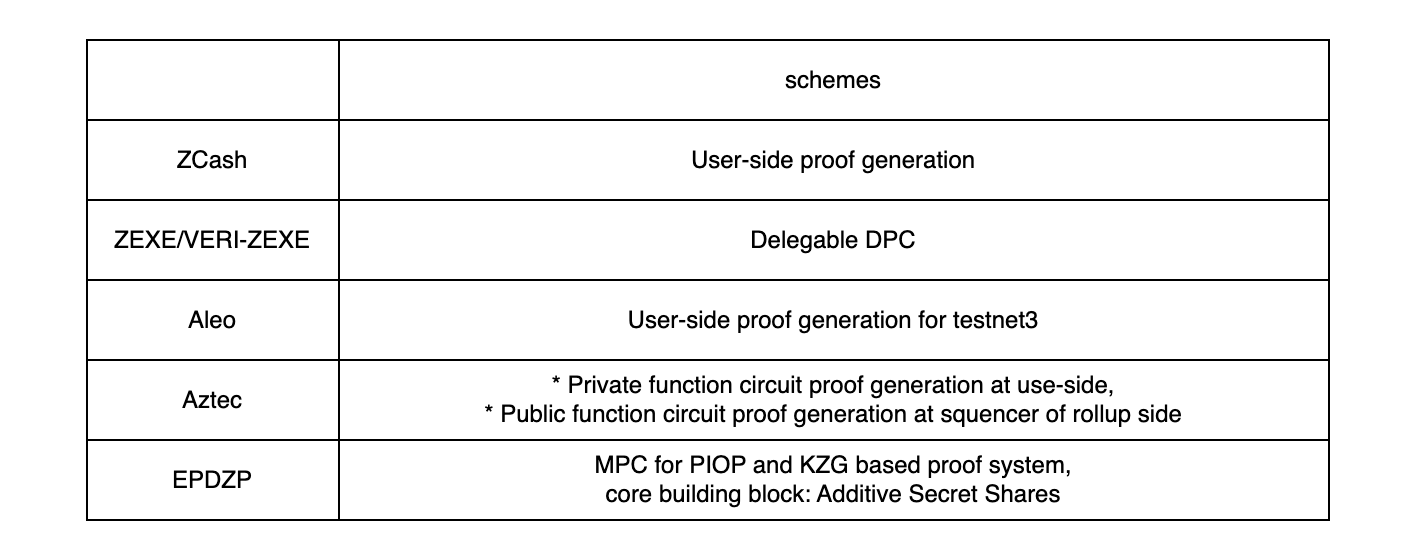
\includegraphics[width=0.6\textwidth]{cur proof generation.jpg}
    \caption{Current Proof Generation Schemes}
    \label{fig:cur_proof_generation}
\end{figure}

As we can see from above figure, ZCash's proof generation scheme is user-side proof generation, which means ZCash has only one type of transaction, which is the transfer of ZEC. The transaction is not complex and the corresponding circuit size is not very large. Therefore, when it comes to proof generation, such as for shielded transactions, it can be done on the user side, for example, generating proofs within a wallet.

The delegable DPC protocol in ZEXE\cite{cryptoeprint:2018/962} allows for the delegation of computations while maintaining security. The protocol involves a delegator who sends input parameters to a delegatee, who then performs an offline computation and generates a proof of correctness using zero-knowledge proofs. The delegatee sends this proof along with the output of the computation back to the delegator, who can use it to generate a transaction that attests to the correctness of the computation. This transaction can be publicly verified by anyone without revealing any additional information about it.

To ensure privacy, ZEXE uses a combination of cryptographic techniques such as zero-knowledge proofs and randomizable signatures. The randomizable signature scheme is used to prevent linking across multiple signatures, which is important for maintaining security in the delegable DPC protocol that the delegatee can not impersonate the delegator, e.g., by producing further transactions that the delegator never authorized.

VERI-ZEXE and ZEXE use the same delegable DPC scheme, we will not repeat it. Aleo's current implementation (testnet3) is still user-side and uses SNARK-powered circuits to generate proofs, but does not yet implement delegable DPC.

Aztec3\cite{website:Aztec3} uses a recursive circuit to generate the final proof, and each contract function is a circuit when a proof needs to be generated. The recursion uses two system circuits, private kernel circuits and public kernel circuits. All private related function calls and their proofs must be entered into private kernel circuits to generate proofs, while all public related function calls and their proofs must be entered into public kernel circuits to generate proofs. In short, the proof of the private circuit is generated on the client side, while the proof of the public circuit is generated in Rollup's Squencer.

Efficient Private Delegation of zkSNARK Provers\cite{website:epdzp} uses MPC to do outsouring proveing. While it keeps witness private and proving efficient, it is designed for Polynomial IOPs and MPC friendly polynomial commitments proof system, while our ZK-ZKVM uses Starky as its internal proof system, which is not suitable for it.

\subsubsection{Our work}

Our design based on ZEXE, and the main procedure of delegable transactions as shown in the figure\ref{fig:delegable_tx} below:

\begin{figure}[!ht]
    \centering
    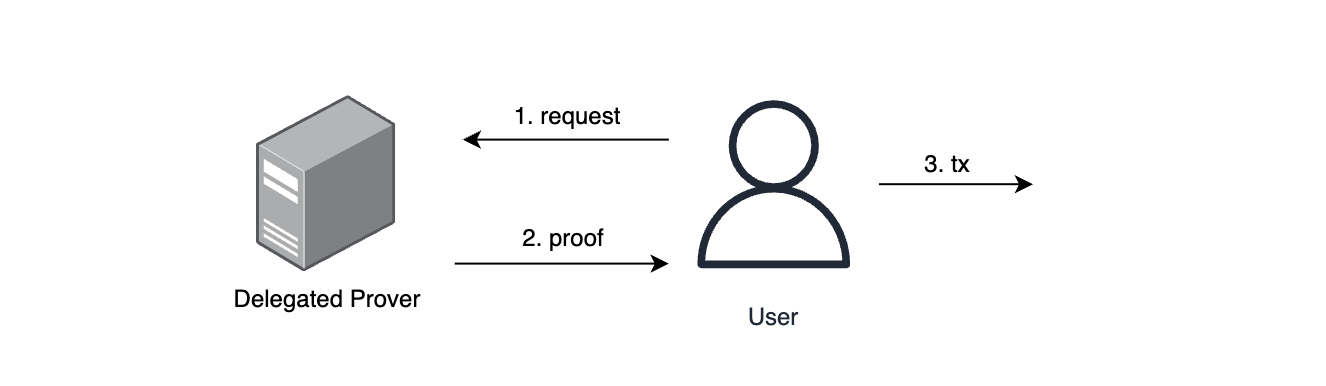
\includegraphics[width=0.6\textwidth]{delegable tx.jpg}
    \caption{Delegable transactions}
    \label{fig:delegable_tx}
\end{figure}

Although ZEXE does not allow the delegatee to impersonate the delegator, the witness remains visible to all participants on the public blockchain. This lack of privacy does not serve our purpose for ZK-ZKVM. To address this issue, we incorporated an external cryptographic primitive called the Secret Share Scheme.

We generate a shared secret by combining the delegatee's public key with the delegator's private key. We then use this shared key to symmetrically encrypt the witness on the delegator's side, and send the encrypted witness to the delegatee. The delegatee uses their private key and the delegator's public key to retrieve the shared key and decrypt the witness.

Once the witness data is decrypted, the subsequent process is identical to that of ZEXE.

Let's say User Alice is the delegator, Prover Bob is the delegatee. We briefly explain our delegable prove scheme:
\color{blue!50!black}
\begin{itemize}
    \item Alice generates shared key $key_{shared} = sk_{alice} \cdot pk_{bob}$
    \item Alice encrypt the witness, the encrypted witness is $witness_{enc} = enc(key_{shared}, witness)$
    \item Alice send the encrypted witness to Bob, while other participants on the public blockchain knows nothing.
    \item Bob generates shared key $key_{shared}' = sk_{bob} \cdot pk_{alice}$, which is same as $key_{shared}$
    \item Bob decrypt the encrypted witness, get raw witness, $witness = dec(key_{shared}', witness_{enc})$
    \item Bob use decrypted witness generating proof $\pi$, send proof back to Alice.
    \item Alice uses her signature private key to construct a transaction within proofs, send it to the blockchain.
\end{itemize}
\normalcolor{}

Our high-level description of our scheme as shown in the figure\ref{fig:our_proof_generation} below:
\begin{figure}[!ht]
    \centering
    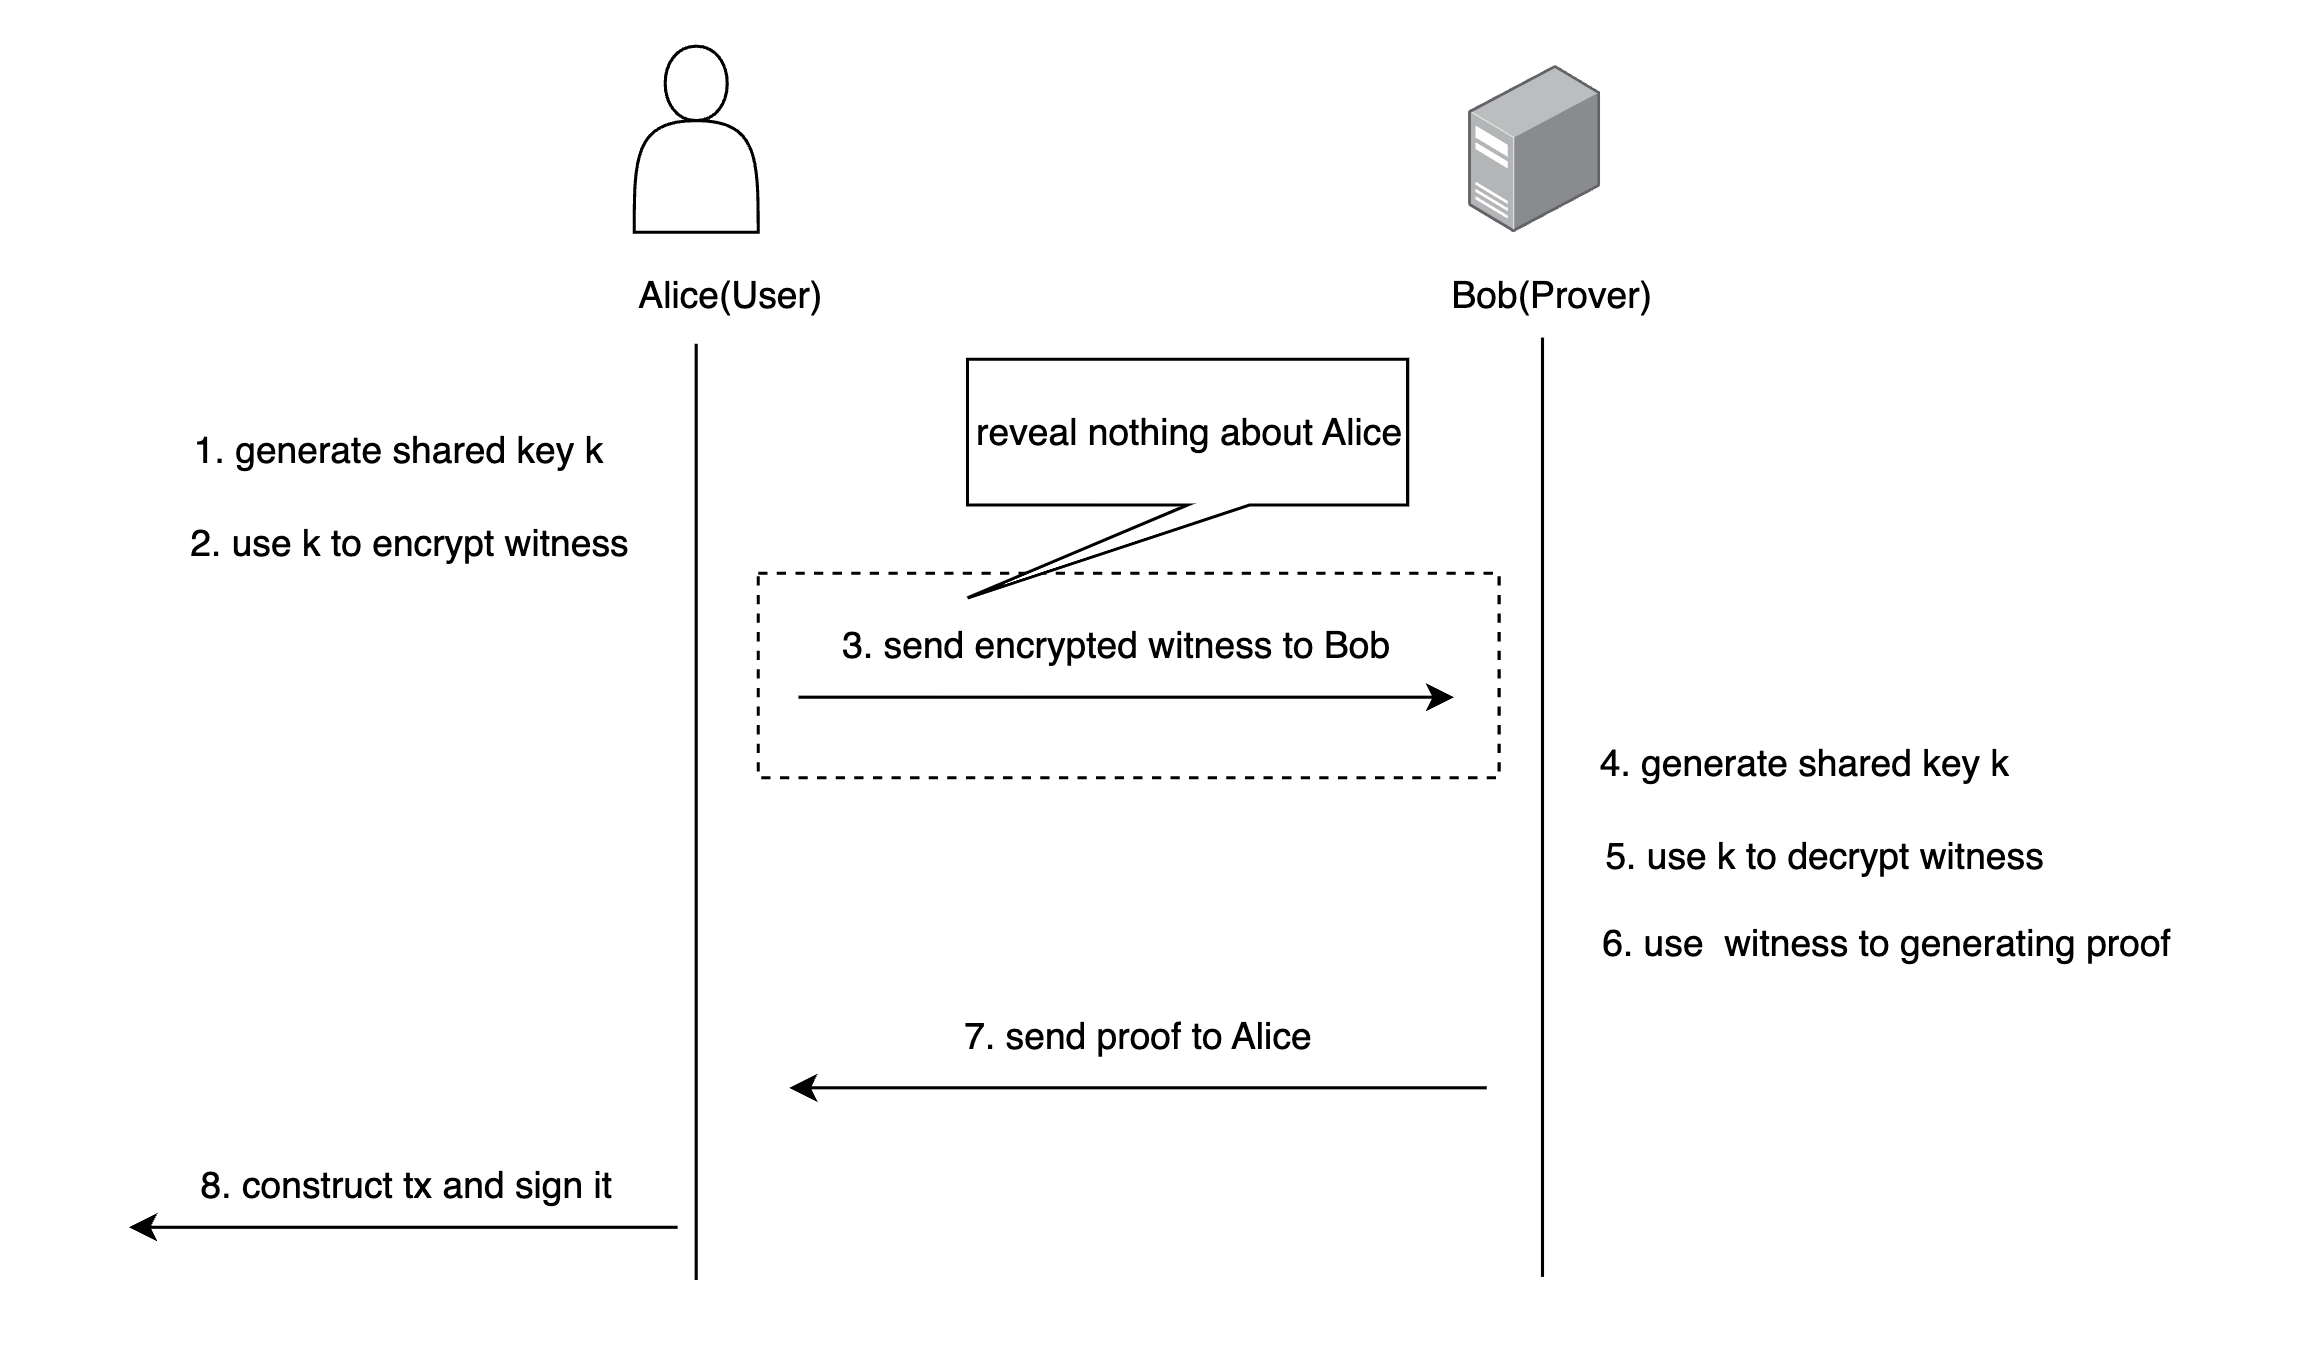
\includegraphics[width=0.6\textwidth]{our proof generation.jpg}
    \caption{Our Proof Generation Scheme}
    \label{fig:our_proof_generation}
\end{figure} 
